\documentclass[12pt, a4paper,
%oneside,      %% -- odkomentujte, pokud chcete svou práci mít pouze jednostrannou, mezera pro hřbet pak automaticky bude pouze na levé straně
twoside,        %% -- pro oboustranné práce, mezera pro hřbet následně střídá strany.
openany
]{report}
%% Nutné balíčky a nastavení
%%%%%%%%%%%%%%%%%%%%%%%%%%%%

%% Proměnné
\newcommand\obor{INFORMAČNÍ TECHNOLOGIE} %% -- napiš číslo a název tvého oboru
\newcommand\kodOboru{18-20-M/01} %% -- napiš číslo a název tvého oboru
\newcommand\zamereni{se zaměřením na počítačové sítě a programování} %% -- napiš číslo a název tvého oboru
\newcommand\skola{Střední škola průmyslová a umělecká, Opava} %% vyplň název školy
\newcommand\trida{IT4} %% vyplň jméno svého konzultanta
\newcommand\jmenoAutora{Michael Meinhard}  %% vyplň své jméno
\newcommand\skolniRok{2023/24} %% vyplň rok
\newcommand\datumOdevzdani{1. 1. 2024} %% vyplň rok
\newcommand\nazevPrace{Dálkově ovládané RC auto přes WiFi} %% vyplň název své práce

\title{\nazevPrace} %% -- Název tvé práce
\author{\jmenoAutora} %% -- tvé jméno
\date{\datumOdevzdani} %% -- rok, kdy píšeš SOČku

\usepackage[top=2.5cm, bottom=2.5cm, left=3.5cm, right=2.5cm]{geometry} %% nastaví okraje, left -- vnitřní okraj, right -- vnější okraj

\usepackage[czech]{babel} %% balík babel pro sazbu v češtině
\usepackage[utf8]{inputenc} %% balíky pro kódování textu
\usepackage[T1]{fontenc}
\usepackage{cmap} %% balíček zajišťující, že vytvořené PDF bude prohledávatelné a kopírovatelné

\usepackage{graphicx} %% balík pro vkládání obrázků

\usepackage{subcaption} %% balíček pro vkládání podobrázků

\usepackage{hyperref} %% balíček, který v PDF vytváří odkazy

\linespread{1.5} %% řádkování
\setlength{\parskip}{1em} %% odsazení mezi odstavci


\usepackage[pagestyles]{titlesec} %% balíček pro úpravu stylu kapitol a sekcí
\titleformat{\chapter}[block]{\scshape\bfseries\LARGE}{\thechapter}{10pt}{\vspace{0pt}}[\vspace{-22pt}]
\titleformat{\section}[block]{\scshape\bfseries\Large}{\thesection}{10pt}{\vspace{0pt}}
\titleformat{\subsection}[block]{\bfseries\large}{\thesubsection}{10pt}{\vspace{0pt}}


\usepackage{tocloft} % Balíček umožní přizpůsobit vzhled tabulky obsahu
\setlength{\cftbeforechapskip}{0pt}  % Menší rozestup pro kapitoly
\setlength{\cftbeforesecskip}{0pt}   % Menší rozestup pro sekce

\setcounter{secnumdepth}{2}
\setcounter{tocdepth}{1}
\usepackage{fancyhdr}
\pagestyle{fancy}
\renewcommand{\headrulewidth}{0.025pt}

\usepackage{booktabs}

\usepackage{url}

%% Balíčky co se můžou hodit :) 
%%%%%%%%%%%%%%%%%%%%%%%%%%%%%%%

\usepackage{pdfpages} %% Balíček umožňující vkládat stránky z PDF souborů, 

\usepackage{upgreek} %% Balíček pro sazbu stojatých řeckých písmen, třeba u jednotky mikrometr. Například stojaté mí: \upmu, stojaté pí: \uppi

\usepackage{amsmath}    %% Balíčky amsmath a amsfonts 
\usepackage{amsfonts}   %% pro sazbu matematických symbolů
\usepackage{esint}     %% pro sazbu různých integrálů (např \oiint)
\usepackage{mathrsfs}
\usepackage{mathptmx} % Times New Roman
\usepackage{hyphenat}

%% makra pro sazbu matematiky
\newcommand{\dif}{\mathrm{d}} %% makro pro sazbu diferenciálu, místo toho
%% abych musel psát '\mathrm{d}' mi stačí napsat '\dif' což je mnohem 
%% kratší a mohu si tak usnadnit práci

\usepackage{listings}
\usepackage{xcolor}

\renewcommand{\lstlistingname}{Kód}% Listing -> Algorithm
\renewcommand{\lstlistlistingname}{Seznam programových kódů}% List of Listings -> List of Algorithms

%% Definice 
\lstdefinelanguage{JavaScript}{
	morekeywords=[1]{break, continue, delete, else, for, function, if, in,
		new, return, this, typeof, var, void, while, with},
	% Literals, primitive types, and reference types.
	morekeywords=[2]{false, null, true, boolean, number, undefined,
		Array, Boolean, Date, Math, Number, String, Object},
	% Built-ins.
	morekeywords=[3]{eval, parseInt, parseFloat, escape, unescape},
	sensitive,
	morecomment=[s]{/*}{*/},
	morecomment=[l]//,
	morecomment=[s]{/**}{*/}, % JavaDoc style comments
	morestring=[b]',
	morestring=[b]"
}[keywords, comments, strings]


\lstdefinelanguage[ECMAScript2015]{JavaScript}[]{JavaScript}{
	morekeywords=[1]{await, async, case, catch, class, const, default, do,
		enum, export, extends, finally, from, implements, import, instanceof,
		let, static, super, switch, throw, try},
	morestring=[b]` % Interpolation strings.
}

\lstalias[]{ES6}[ECMAScript2015]{JavaScript}

% Nastavení barev
% Requires package: color.
\definecolor{mediumgray}{rgb}{0.3, 0.4, 0.4}
\definecolor{mediumblue}{rgb}{0.0, 0.0, 0.8}
\definecolor{forestgreen}{rgb}{0.13, 0.55, 0.13}
\definecolor{darkviolet}{rgb}{0.58, 0.0, 0.83}
\definecolor{royalblue}{rgb}{0.25, 0.41, 0.88}
\definecolor{crimson}{rgb}{0.86, 0.8, 0.24}

% Nastavení pro Python
\lstdefinestyle{Python}{
	language=Python,
	backgroundcolor=\color{white},
	basicstyle=\ttfamily,
	breakatwhitespace=false,
	breaklines=false,
	captionpos=b,
	columns=fullflexible,
	commentstyle=\color{mediumgray}\upshape,
	emph={},
	emphstyle=\color{crimson},
	extendedchars=true,  % requires inputenc
	fontadjust=true,
	frame=single,
	identifierstyle=\color{black},
	keepspaces=true,
	keywordstyle=\color{mediumblue},
	keywordstyle={[2]\color{darkviolet}},
	keywordstyle={[3]\color{royalblue}},
	literate=%
	{á}{{\'a}}1 {č}{{\v{c}}}1 {ď}{{\v{d}}}1 {é}{{\'e}}1 {ě}{{\v{e}}}1
	{í}{{\'i}}1 {ň}{{\v{n}}}1 {ó}{{\'o}}1 {ř}{{\v{r}}}1 {š}{{\v{s}}}1
	{ť}{{\v{t}}}1 {ú}{{\'u}}1 {ů}{{\r{u}}}1 {ý}{{\'y}}1 {ž}{{\v{z}}}1,		
	numbers=left,
	numbersep=5pt,
	numberstyle=\tiny\color{black},
	rulecolor=\color{black},
	showlines=true,
	showspaces=false,
	showstringspaces=false,
	showtabs=false,
	stringstyle=\color{forestgreen},
	tabsize=2,
	title=\lstname,
	upquote=true  % requires textcomp	
}


\lstdefinestyle{JSES6Base}{
	backgroundcolor=\color{white},
	basicstyle=\ttfamily,
	breakatwhitespace=false,
	breaklines=false,
	captionpos=b,
	columns=fullflexible,
	commentstyle=\color{mediumgray}\upshape,
	emph={},
	emphstyle=\color{crimson},
	extendedchars=true,  % requires inputenc
	fontadjust=true,
	frame=single,
	identifierstyle=\color{black},
	keepspaces=true,
	keywordstyle=\color{mediumblue},
	keywordstyle={[2]\color{darkviolet}},
	keywordstyle={[3]\color{royalblue}},
 literate=%
{á}{{\'a}}1 {č}{{\v{c}}}1 {ď}{{\v{d}}}1 {é}{{\'e}}1 {ě}{{\v{e}}}1
{í}{{\'i}}1 {ň}{{\v{n}}}1 {ó}{{\'o}}1 {ř}{{\v{r}}}1 {š}{{\v{s}}}1
{ť}{{\v{t}}}1 {ú}{{\'u}}1 {ů}{{\r{u}}}1 {ý}{{\'y}}1 {ž}{{\v{z}}}1,		
	numbers=left,
	numbersep=5pt,
	numberstyle=\tiny\color{black},
	rulecolor=\color{black},
	showlines=true,
	showspaces=false,
	showstringspaces=false,
	showtabs=false,
	stringstyle=\color{forestgreen},
	tabsize=2,
	title=\lstname,
	upquote=true  % requires textcomp
}

\lstdefinestyle{JavaScript}{
	language=JavaScript,
	style=JSES6Base,
}
\lstdefinestyle{ES6}{
	language=ES6,
	style=JSES6Base
}


\usepackage{lipsum} %% balíček který píše lipsum (nesmyslný text, který se používá pro kontrolu typografie)

%% Začátek dokumentu
%%%%%%%%%%%%%%%%%%%%
\begin{document}
    \pagestyle{empty}
	\clearpage

%% Titulní stránka s informacemi
%%%%%%%%%%%%%%%%%%%%%%%%%%%%%%%%%%%%%%%%
	
	{\fontfamily{phv}\selectfont
		%% Logo školy
		\begin{figure}[h]
			\centering
			
\includegraphics[width=0.6\linewidth]{image/logo-skoly.png} 
		\end{figure}
		
		
		%% Hlavička práce a její název (viz proměnná \nazev prace)
		%% \sffamily %%% bezpatkové písmo - sans serif
		{\bfseries %%% písmo na stránce je tučně
			\begin{center}
				\vspace{0.025 \textheight}
				\LARGE{ZÁVĚREČNÁ STUDIJNÍ PRÁCE}\\
				\large{dokumentace}\\
				\vspace{0.075 \textheight}
				\LARGE {\nazevPrace}\\
			\end{center}  
		}%%%
		
		\begin{figure}[h]
			\centering
			
\includegraphics[width=0.8\linewidth]{image/programovani-02.jpg} 
		\end{figure}
		
		\vspace{0.02 \textheight}
		\begin{table}[h!]
			\begin{tabular}{ll}
				\textbf{Autor:} & \jmenoAutora\\ 
				\textbf{Obor:} & \kodOboru { } \obor\\
				\textbf{} & \zamereni\\
				\textbf{Třída:} & \trida\\
				\textbf{Školní rok:} & \skolniRok\\
			\end{tabular}
			
		\end{table}		
	}	
\clearpage
	
%% Stránka obsahující poděkování a prohlášení
%%%%%%%%%%%%%%%%%%%%%%%%%%%%%%%%%%%%%%%%%%%%%%%%%%%%%%%%
%% Poděkování - nepovinné
%%%%%%%%%%%%%%%%%%%%%%%%%%%%
	
	\noindent{\large{\bfseries{Poděkování}\\}}
	\noindent Děkuji panu učiteli Mgr. Marcelu 
Godovskému za jeho doporučení a půjčení testovacích součástek a panu učiteli Mgr. Markovi Lučnému za cené rady s webem.
	
	\vspace*{0.6\textheight} %% Vertikální mezeru je možné upravit

%% Prohlášení - povinné
%%%%%%%%%%%%%%%%%%%%%%%%%%%%
	\noindent{\large{\bfseries{Prohlášení}\\}}  %% uprav si koncovky podle toho na jaký rod se cítíš, vypadá to pak lépe :) 
	\noindent{Prohlašuji, že jsem závěrečnou práci vypracoval samostatně a uvedl veškeré použité 
		informační zdroje.\\}
	\noindent{Souhlasím, aby tato studijní práce byla použita k výukovým a prezentačním účelům na Střední průmyslové a umělecké škole v Opavě, Praskova 399/8.}
	\vfill
	\noindent{V Opavě \datumOdevzdani\\}
	\noindent
	\begin{minipage}{\linewidth}
		\hspace{7.5cm} 
		\begin{tabular}{@{}p{6cm}@{}}
			\dotfill \\
		Podpis autora
		\end{tabular}
	\end{minipage}
	
	\clearpage %% Zalomení

%% Stránka obsahující abstrakt (anotaci)
%%%%%%%%%%%%%%%%%%%%%%%%%%%%%%%%%%%%%%%%%%%%%%%%%%%%%%%%	
	\noindent{\Large{\bfseries{Abstrakt}\\}}
	\noindent Tento projekt se zabývá vytvoření RC auta s využitím vývojové desky ESP32-CAM a Arduina. Hlavním cílem bylo implementovat možnost dálkového ovládání vozidla přes WiFi a přenosu obrazu z kamery. Přestože jsem úspěšně vytvořil funkční RC auto s manuálním ovládáním a sledováním, nezakomponoval jsem zde detekci překážek a automatický pohyb. Budoucí plány směřují k rozšíření těchto funkcí.
 
  \noindent Komunikace s RC autem probíhá přes WiFi, kde uživatel zadává heslo k připojení. Po úspěšném připojení k síti pomocí mobilu nebo počítače zadává IP adresu, čímž se připojuje na server RC auta. Na obrazovce se okamžitě zobrazuje živý obraz z kamery, spolu s šipkami umožňujícími ovládání pohybu vozidla. Uživatel tak může intuitivně a v reálném čase ovládat RC auto prostřednictvím svého zařízení.
	
	\vspace{18pt}
	
	\noindent{\large{\bfseries{Klíčová slova}}}
	
	\noindent RC auto, ESP32-CAM, Arduino, WiFi, vzdálené ovládání, kamera
    \clearpage
%% Stránka s generovaným obsahem
%%%%%%%%%%%%%%%%%%%%%%%%%%%%%%%%%%%%%%%	
        \setcounter{tocdepth}{3}  % Zahrnuje subsekce do obsahu
        \setcounter{secnumdepth}{3}  % Čísluje subsekce
        \fancypagestyle{originalplain}{
  \fancyhf{}
  \fancyfoot[C]{\thepage} % Example: put page number at center of footer.
  \renewcommand{\headrulewidth}{0pt}
  \renewcommand{\footrulewidth}{0pt}
}

% Redefine the 'plain' page style to be empty
\fancypagestyle{plain}{
  \fancyhf{} % clear all header and footer fields
  \renewcommand{\headrulewidth}{0pt}
  \renewcommand{\footrulewidth}{0pt}
}
        \tableofcontents %% Vygeneruje tabulku s obsahem
        \clearpage
% Restore the standard 'plain' page style immediately after the ToC
\fancypagestyle{plain}{%
  % Restore the original 'plain' style definitions
  \fancyhf{}
  \fancyfoot[C]{\thepage} % Example: put page number at center of footer.
  \renewcommand{\headrulewidth}{0pt}
  \renewcommand{\footrulewidth}{0pt}
}
% Reset the page style to your preferred style for subsequent pages
\pagestyle{originalplain} % or 'originalplain' if you want to use the saved 'plain' style    
%% Stránka s úvodem - povinná část
%%%%%%%%%%%%%%%%%%%%%%%%%%%%%%%%%%%%%%%
	\chapter*{Úvod}
	\addcontentsline{toc}{chapter}{Úvod}
%Tento příkaz ručně přidává záznam do obsahu.
%První parametr toc označuje, že přidáváme záznam do Table of Contents (obsahu).
%Druhý parametr chapter specifikuje úroveň záznamu. V tomto případě říkáme, že přidávaný záznam má být považován za kapitolu.
%Třetí parametr Úvod je text, který se objeví v obsahu. V tomto případě bude v obsahu zobrazen název "Úvod".
\noindent Od dětství mě fascinovala RC auta. Mým dlouholetým snem bylo sestavit vlastní RC auto a prozkoumat, jak mohu tuto technologii využít. Rozhodl jsem se uskutečnit svou touhu sestavit RC auto s možností ovládání přes WiFi a přenosem obrazu z kamery.

\noindent Cílem tohoto projektu bylo nejen vytvořit plně funkční RC auto, ale také se naučit proces sestavení a zapojení komponent. Klíčovou částí mé práce bylo propojení RC auta s WiFi serverem, což umožňuje vzdálené ovládání a sledování prostřednictvím kamery.

\noindent Během této dokumentace zahrnu sestavení RC auta, implementaci WiFi serveru a integraci kamery. Momentálně auto umožňuje ruční ovládání a sledování terénu. Mým plánem do budoucna je rozšířit funkcionalitu auta o detekci překážek a možnost automatického pohybu. Uvědomuji si, že tato funkce přinese další rozměr a zajímavost do projektu. V závěru se zaměříme na současný stav projektu, popsání dosažených cílů a ohodnocení odvedené práce.

%Tipy k psaní úvodu
%Je povinný, nadpis neměňte, rozsah - max. 1 strana. 
%Tato část práce obsahuje: 
%* náhled do řešené problematiky, zdůvodnění volby problematiky, 
%* předem definované cíle práce, 
%* motivaci pro další čtení textu včetně stručného uvedení obsahu následujících kapitol 

\pagestyle{plain}
\chapter{VÝROBA A SESTAVENÍ RC MODELU}
\noindent Celý proces výroby a sestavování RC modelu započal výběrem vhodných součástek, což pro mě jako nováčka v tomto odvětví zabralo spoustu času. Musel jsem pečlivě vybírat, abych zajistil, že všechny součástky budou vzájemně kompatibilní a celý model bude spolehlivě fungovat.

\noindent Původní plán vytisknout model auta 3D tiskárnou se změnil, když jsem objevil existující model, který nejenže splňoval mé požadavky, ale obsahoval i některé z potřebných součástek. To mi z části ušetřilo čas a zjednodušilo celý proces.

\noindent Sestavování bylo krok po kroku, součástka po součástce. Dával jsem pozor na každý detail, aby vše bylo správně připojeno a pevně drželo. Ostatní součástky jsem testoval předtím, než jsem je úplně zapojil, abych se vyhnul pozdějším potížím.

\noindent Až poté, co bylo vše fyzicky spojeno, přišla na řadu fáze programování. Začal jsem s jednoduchými příklady pro zobrazení obrazu z kamery. Pro programování jsem použil jazyk Arduino, což je kombinace jazyku C a C++. Na komunikaci s webem jsem potřeboval speciální balíčky, například AsyncTCP, který tvořil základ pro ESPAsyncWebServer. Design webového rozhraní jsem upravil s pomocí HTML, CSS a dalších technologií, které mi ulehčili zpříjemnit vzhled stránky.

\chapter{PRINCIP VZDÁLENÉHO OVLÁDÁNÍ}
\noindent Mým primárním cílem bylo navázat bezdrátovou komunikaci prostřednictvím WiFi. K tomu jsem využil mikrokontrolér ESP32 a Arduino, kde Arduino plnilo roli programátoru pro nahrávání kódu do ESP32. Zásadním krokem bylo vytvoření spojení se serverem. Ovladač (mobilní zařízení nebo počítač) se připojí k serveru přes WiFi po zadání přístupových údajů (hesla) se naváže spojení umožňující zadat IP adresu do prohlížece a zahájit komunikaci mezi ovladačem a modelem RC auta.

\noindent Implementace ovládání vozidla byla následným krokem, kde na webovém rozhraní byla integrována šipková tlačítka umožňující pohyb vozidla vpřed, vzad, doprava a doleva. To vytvořilo intuitivní a snadno ovladatelný systém.


\chapter{VYUŽITÉ TECHNOLOGIE}

\section{HARDWARE}

V této kapitole se seznámíme s použitým hardware.

\subsection{Seznam součástek}
\begin{itemize}
    \item Vývojová deska ESP32-CAM,
    \item H můstek L298N Dual H Most DC,
    \item Arduino MEGA 2560 Rev3,
    \item Hadex motorek 3-6V/0,17A s převodovkou, převod 1/48
    \item snímač otáček
    \item nepájivé pole
\end{itemize}

\subsection{ESP32-CAM}
\noindent Základem mého projektu byla vývojová deska ESP32-CAM (obrázek č. 1). Poskytla mi opravdu skvělý způsob jak přidat vizuální prvek do mého projektu. Tato deska spojuje výkonný mikrokontrolér ESP32 s kamerovým modulem, což umožňuje snadné zachycení a zpracování obrazu. Díky flexibilním GPIO pinům, podpoře pro paměťové karty a jednoduchému programování pomocí Arduino IDE poskytuje ideální řešení pro mé potřeby. S integrovanou WiFi podporou je snadné přenášet data bezdrátově, což rozšiřuje možnosti komunikace a přenosu informací.
\begin{figure}
    \begin{subfigure}{0.48\textwidth}
        \centering
		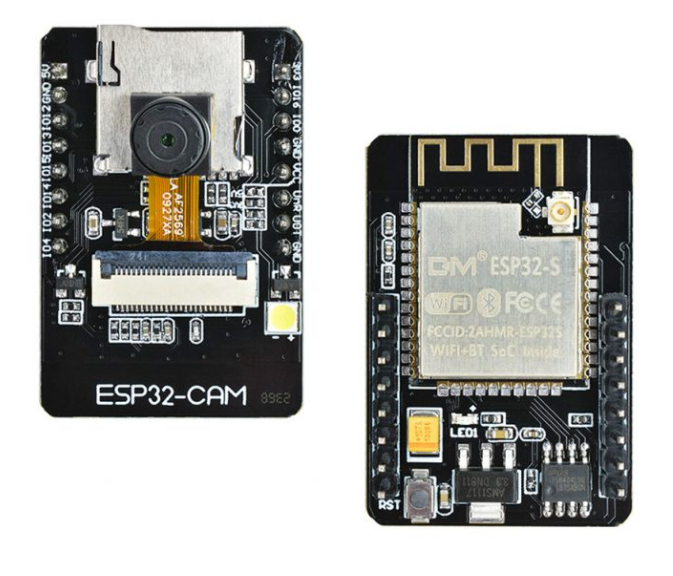
\includegraphics[width=\textwidth]{image/esp32.png}
        \caption*{\textit{obrázek č. 1 ESP32-CAM}}
        \label{fig:esp32}
    \end{subfigure}
    \begin{subfigure}{0.48\textwidth}
        \centering
        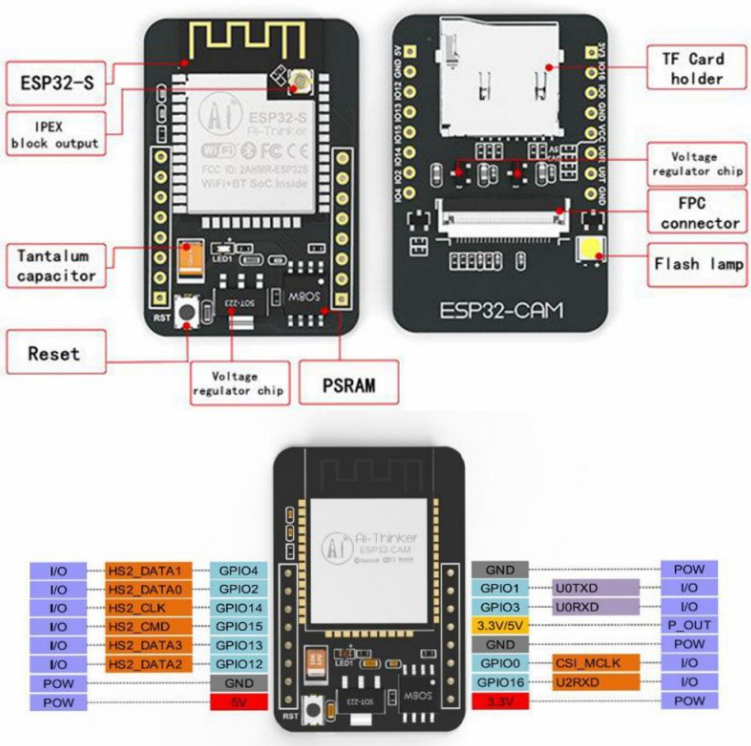
\includegraphics[width=\textwidth]{image/esp32-pins.png}
        \caption*{\textit{obrázek č. 2 Piny ESP32-CAM}}
    \end{subfigure}     
\end{figure}

\subsection{L298N Dual H Most DC}
\noindent V rámci mého projektu RC auta se H-můstek L298N stal důležitou součástí pro pohyb DC motorů. Jeho snadné zapojení a schopnost nezávislého ovládání obou motorů dodaly projektu potřebnou variabilitu pro dosažení plynulého pohybu vozidla.

\noindent Během integrování H-můstku L298N do celkového systému jsem ocenil jeho přehledný design a spolehlivost. Jeho spolupráce s mikrokontrolérem umožnila programovat pohyb motorů tak, jak jsem si představoval. Vyzkoušel jsem i možnosti stanovení rychlosti motorů.

\subsection{Arduino MEGA 2560 Rev3}
Hlavní výhodou používání.

\subsection{Hadex motorek 3-6V/0,17A}
Hlavní výhodou používání.

\section{SOFTWARE}
V této kapitole se podíváme na použitým software.

\subsection{Použitý jazyk}
Preambule je první částí každého.

\subsection{Arduino IDE}
Preambule je první částí každého.

\subsection{Web Server}
Preambule je první částí každého.

\subsection{WebSocket komunikace}
Pokracuj textem zde.

\chapter{POUŽITÉ POSTUPY A ŘEŠENÍ}

\section{HARDWARE TECHNOLOGIE}

\subsection{Schéma}
napis zde.


\subsection{Nahrávání kódu}
napis zde.

\subsection{Zoptimálnění funkčnosti ESP32-CAM}
napis zde.


	\section[Základy]{Základy: Text, obrázky, tabulky a citace} %%[Text, který bude v obsahu]{Text, který se vytiskne na stránce} Zkus měnit jednotlivé závorky a uvidíš :) 
	Psaní v \LaTeX{u} není žádná věda, stačí psát normálně do zdrojového souboru. Pokud bys chtěl psát obrážky či číslovaný seznam, pak můžeš použít prostředí \texttt{itemize} či \texttt{enumerate}. Často je důležité používat nezlomitelnou mezeru. Tu uděláš pomocí \verb|~|~(tildy). Pokud budeš chtít psát uvozovky použij příkaz \texttt{uv}, pomocí něj se ti vytvoří uvozovky podle příslušného jazyka. V česku tedy ve formátu 99 66. Použití příkazu najdeš níže v textu.
	
	Občas je zapotřebí \LaTeX{u} pomoct při rozdělování slov. To se udělá snadno vložením symbolů \verb|\-| mezi jednotlivé slabiky.
	
	\subsection{Tabulky}
	
	U tabulek platí to stejné co u obrázků. Zarovnávají se na střed a nechávají se \uv{plavat} v textu. Tabulka narozdíl od textu, má popisek nahoře. U tabulky \ref{tab:ukazka} je použit balíček \texttt{booktabs}, pomocí kterého je celá tabulka naformátovaná.
	
	Seznam jak obrázků tak tabulek je pak vytvořen pomocí příkazů \texttt{listoftables} a~\texttt{list\-of\-fig\-ures} na konci práce před literaturou.
	
	\begin{table}[h]
		\caption{Tato tabulka slouží jako ukázka toho, jak mohou tabulky vypadat.} %% popisek se u tebaluky píše nad ní
		\label{tab:ukazka} %% označení pro pozdější odkazování se 
		\centering
		\begin{tabular}{lll}
			\toprule %% příkazy z balíčku booktabs
			záhlaví& této & tabulky\\
			\midrule
			obsah&tabulky& už\\
			není & oddělený &čarami\\
			\bottomrule
		\end{tabular}
	\end{table}
	
	
	\subsection{Obrázky}
	
	U obrázků je dobré používat vektorové formáty, pokud to jde. \LaTeX se nejvíc kamarádí s formátem PDF. Do známého PDFka lze z jiných vektorových formátů (ať už SVG či ESP) obrázky přenést snadno pomocí grafických programů, jako je třeba Inkscape. \LaTeX si rozhodně poradí i s tradičními formáty PNG a JPG, avšak tyto obrázky mohou zabírat více prostoru a při tisku se může projevit nižší rozlišení obrázků. Pokud chceš používat tyto obrázky, rozhodně měj na paměti, aby měli rozlišení alespoň 250 indálně 330 ppi.
	
	Obrázky se vkládají do prostředí \texttt{figure}, při úpravě šířky je možné krom tradičních jednotek jako cm nebo mm použít také jako jednotku šířku stránky \texttt{textwidth} to se hodí zejména když chceš mít více podobrázků. 
	
	U každého obrázku je důležité aby měl popisek, \texttt{caption}. Do popisku napiš, co na obrázku je, případně nějaký další popis, tak aby čtenář následně neměl sebemenší pochybnost. U obrázků co nejsou tvoje nezapomeň an citaci. Jinak by to totiž znamenalo, že jsi obrázek dělal ty sám, což není etické přivlastňovat si cizí díla. Popisek obrázku je věta, proto musí vždy končit tečkou.
	
	\begin{figure}[h!]
		\centering %% příkaz, který ti obrázek zarovná na střed
		
\includegraphics[width=0.6\textwidth]{image/logo-skoly.png} %% vložení samotného obrátku
		\caption{Logo SŠPU Opava \cite{sspuLogo}.} %% popisek obrázku, nezapomeň na citace!
		\label{fig:logoSSPU} %% označení až budeš chtít na obrázek odkazovat
	\end{figure}
	
	Když chceš odkazovat na obrázek, stačí pak už jen napsat příkaz \texttt{ref} a do závorek napsat označení obrázku. Třeba logo SOČky, můžeš vidět na obrázku \ref{fig:logoSSPU} \cite{socSSPU}.
	
	
	\begin{figure}[h!] \centering
		\begin{subfigure}[h]{0.63\textwidth} %%prostředí pro podobrázek {šířka podobrázku}
			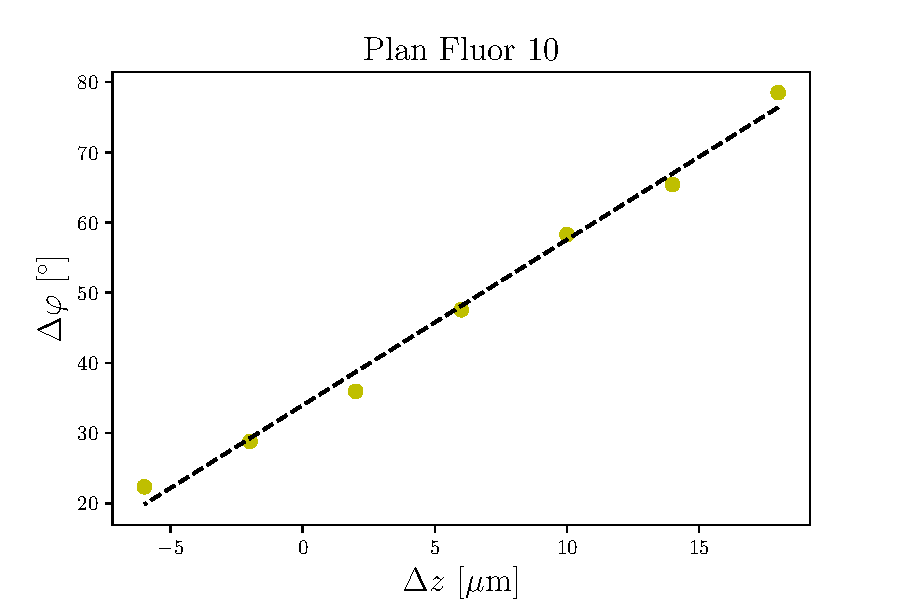
\includegraphics[width=\textwidth]{image/vysledek_10} 
			\caption{} %% aby se ti vysázelo označení obrázku.
		\end{subfigure}
		\begin{subfigure}[h]{0.63\textwidth}
			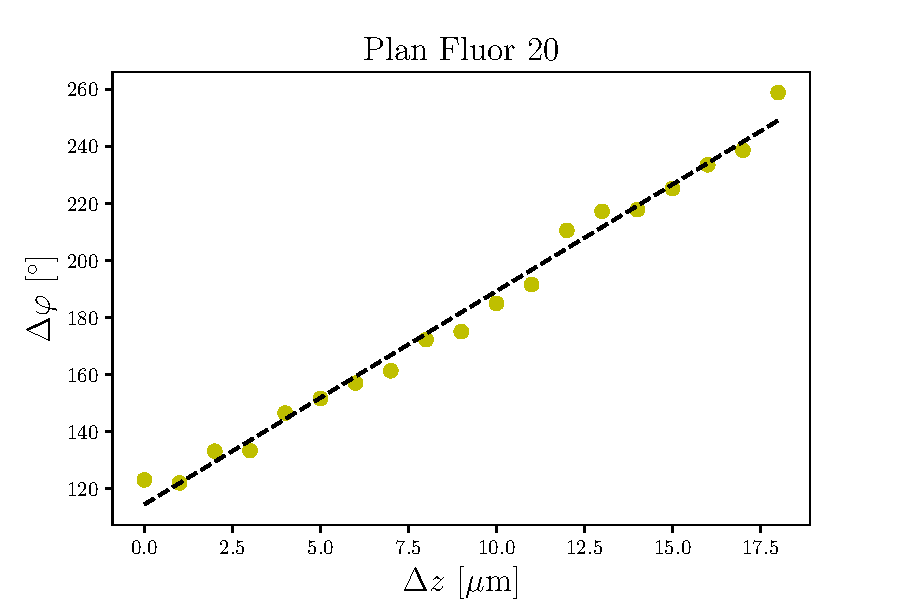
\includegraphics[width=\textwidth]{image/vysledek_20}
			\caption{}
		\end{subfigure}
		\caption[Graf závislosti rotace DH PSF $\Delta\varphi$ na defokusaci objektivu $\Delta z$.]{Graf závislosti rotace DH PSF $\Delta\varphi$ na defokusaci objektivu $\Delta z$, (a) při použití objektivu Plan Fluor 10, (b) při použití objektivu Plan Fluor 20. Měřená data (žluté body) jsou lineárně proloženy (přerušovaná přímka). }
		\label{fig:rotace_grafy}
	\end{figure}
	
		Pokud bys měl více podobrázků přichází do hry balíček \texttt{subcaption}. Pomocí něj lze vysázet i podobrázky. U podobrázků se popisek píše pouze jeden, dolů. Je v tomto připadě vhodné použít navíc hranaté závorky, do nichž se napíše kratší popisek, který se následně ukáže v seznamu obrázků.
	
	Všimni si, že obrázky jsou naschvál široké. Je to proto, aby byly dobře čitelné. Také si všimni popisku grafů. Ačkoli nejspíš netušíš co je to DH PSF či defokusace objektivu mělo by ti být jasné, že je důležité přesně graf popsat. To znamená co je na vodorovné ose, co je na svislé ose. V jakých jednotkách veličiny jsou. Které body co znamenají, která křivka má jaký význam. Napsat samotné \uv{$\Delta \varphi$} je málo, vždy raději připoměň, co daná značka znamená.
	

	
	\subsection{Literatura}
	
	V \LaTeX{}u lze dělat seznam literatury dvěma způsoby. V této šabloně jsem použil ten, kdy se seznam literatury píše přímo do práce. Pro jeho vygenerování doporučuji použít některý z generátarů, jako jsou například Citace PRO \cite{citacePRO}. Pomocí citací lze vygenerovat přímo dokument, který se pak už jen překopíruje do textu a člověk nemusí nic zvýrazňovat. Dále lze využít Bibtex, který rozhodně do budoucna hodlám zaimplementovat do šablony, avšak jeho použití nemusí být tak přátelské k začátečníkům.
	
	Pokud bys chtěl odkazovat na vícero zdrojů stačí je napsat vedle sebe oddělené čárkou \cite{LaTeXprirucka, citacePRO, Born2019}. Případně můžu odkaz na konkrétní stránku dát do hranatých závorek, viz \cite[str.~1]{Born2019}
	
	\subsection{Programový kód}
	Pro vložení programového kódu do dokumentu LaTeX s možností zvýraznění syntaxe můžete použít balíček \texttt{listings}. Tento balíček nabízí široké možnosti pro formátování kódu, včetně zvýraznění syntaxe pro různé programovací jazyky.
	
	Nejprve je třeba do preambule LaTeX dokumentu přidat \texttt{\\usepackage{listings}} a nastavit příslušné parametry. Příklad nastavení pro jazyk Python by mohl vypadat takto:
	

\begin{lstlisting}[style=Python, caption={Ukázka Python kódu}]
	# Python code here
	def hello_world():
		print("Hello, world!")
\end{lstlisting}


\begin{lstlisting}[style=JavaScript, title={Kód}, caption={Ukázka JS kódu}]
	// JavaScript code here
	function helloWorld() {
		console.log("Hello, world!");
	}
\end{lstlisting}	
	
\begin{lstlisting}[style=ES6, caption={ES6 (ECMAScript-2015) Listing}]
	/* eslint-env es6 */
	/* eslint-disable no-unused-vars */
	
	import Axios from 'axios'
	import { BASE_URL } from './utils/api'
	import { getAPIToken } from './utils/helpers'
	
	export default class User {
		constructor () {
			this.id = null
			this.username = null
			this.email = ''
			this.isActive = false
			this.lastLogin = ''  // ISO 8601 formatted timestamp.
			this.lastPWChange = ''  // ISO 8601 formatted timestamp.
		}
	}
	
	const getUserProfile = async (id) => {
		let user = new User()
		await Axios.get(
		`${BASE_URL}/users/${id}`,
		{
			headers: {
				'Authorization': `Token ${getAPIToken()}`,
			}
		}
		).then{response => {
				// ...
			}).catch(error => {
				// ...
			})
		}
\end{lstlisting}	
	
	\section[Pokročilejší tipy]{Pokročilejší tipy, které se mohou hodit}
	
	\subsection{Rovnice}
	
	Sazba matematiky je věda sama o sobě. Ačkoli Word prošel obrovskou změnou a je v~tomto mnohem lepší, tak \LaTeX je pro to přímo (ještě jsem neviděl matematika, co by používal Word). Spolu s balíčky \texttt{amsmath} a \texttt{amsfonts} snad neexistuje nic, co by se používalo a \LaTeX by to nezvládl. Ať už jde o základní věci jako řecká písmenka -- $\alpha, \beta, \gamma, \dots$ -- integrály -- $\int_{l_i}^{l_f} \tau \dif l $ -- až třeba po speciální písmena -- $\mathscr{F}: \mathbb{R}^n \to \mathbb{R}^m$. Pro případ, že bys potřeboval nějaké speciální integrály, je tu balíček \texttt{esint}, pomocí něj můžeš napsat třeba
	$$ \oiint_{S(V)} \vec{E} \cdot \dif \vec{S} = \iiint_{V} \left(\vec{\nabla} \cdot \vec{E}\right) \dif V .$$
	
	Jak můžeš vidět tak rovnice lze psát jednak do textu a nebo pokud se jedná o nějakou důležitou nebo rozsáhlejší rovnici tak na samostatný řádek. Pokud je rovnice opravdu důležitá, tak je vhodné ji také číslovat. Pak se na ni můžeš dále odkazovat v textu.
	\begin{equation}
		\vec{F} = m \vec{a}
		\label{eq:newton2}
	\end{equation}
	\dots Například podle druhého Newtonova zákona, rovnice (\ref{eq:newton2}) \dots Zároveň je vždy nutné vysvětlit co která veličina znamená. V tomto případě bych napsal, že v druhém Newtonově zákoně vektor síly $\vec F$ odpovídá součinu hmotnosti tělesa $m$ a jeho zrychlení $\vec a$. 
	
	Věřím, že se sazbou matematiky ti pomůže tvůj školitel, případně mi můžeš napsat (mail je v úvodu). Jednotlivé funkcionality spolu se seznamem znaků nalezneš jednak v Ne příliš stručném úvodu~\cite{LaTeXprirucka} nebo na Wikibooks v sekcích \emph{Mathematics} a \emph{Advanced mathematics}~\cite{wikibooksLaTeX}.
	
	
	
	
	\chapter{Když dokončuji práci}
	
	Každou práci je dobré zkontrolovat, aby v ní nebyly pravopisné chyby, nebyla těžkopádně napsaná -- byla čtivá -- a neobsahovala žádný typografický nedostatek. Proto, když práci sepíšeš, nech ji chvilku odležet, třeba týden. Pak si ji po sobě znovu přečti. Hned uvidíš, kolik věcí bys napsal jinak případně kde tě bije do očí jaká chyba. Dej práci přečíst také svému školiteli a případně češtináři. Zajistíš tak, že bude obsahovat méně chyb.
	
	Pak můžeš práci vytisknout a hurá do soutěže.
	
	\chapter*{Závěr}
	
	Věřím, že jsem ti spolu se šablonou poskytl několik tipů, jak napsat práci. Ať už jde o úplné začátky s \LaTeX{}em. Či ukázku toho, co vše s ním zvládneš. Pokud bys měl k šabloně libovolné dotazy, rouhodně se na mě obrať. \LaTeX tvé práci dodá určitou krásu, tak doufám, že ti dodá sebevědomí a uspěješ při souteži. A i kdyby ne vzpomeň si, kolik ses toho musel naučit a hned uvidíš o jaký kus ses posunul.
	
	%% literatura
	\begin{thebibliography}{99}
		\bibitem{sablonaSOC} DOKULIL Jakub. \textit{Šablona pro psaní SOČ v programu \LaTeX} [Online]. Brno, 2020 [cit. 2020-08-24]. Dostupné z: \url{https://github.com/Kubiczek36/SOC_sablona}
		\bibitem{LaTeXprirucka}OETIKER, Tobias, Hubert PARTL, Irene HYNA, Elisabeth SCHEGL, Michal KOČER a Pavel SÝKORA. \textit{Ne příliš stručný úvod do systému LaTeX2e} [online]. 1998 [cit. 2020-08-24]. Dostupné z: \url{https://www.jaroska.cz/elearning/informatika/typografie/lshort2e-cz.pdf}
		\bibitem{wikibooksLaTeX}\textit{Wikibooks: LaTeX} [online]. San Francisco (CA): Wikimedia Foundation, 2001- [cit. 2020-08-24]. Dostupné z: \url{https://en.wikibooks.org/wiki/LaTeX}
		\bibitem{stackExchange} \textit{TeX - LaTeX Stack Exchange} [online]. Stack Exchange, 2020 [cit. 2020-09-01]. Dostupné z: \url{https://tex.stackexchange.com}
		\bibitem{sspuLogo} \textit{Střední škola průmyslová a umělecká Opava} [online]. [cit. 2023-11-11]. Dostupné z: \url{https://www.sspu-opava.cz}
		\bibitem{citacePRO}\textit{Citace PRO} [online]. Citace.com, 2020 [cit. 2020-08-31]. Dostupné z: \url{https://www.citacepro.com}
		\bibitem{Born2019} BORN, Max a Emil WOLF. \textit{Principles of optics: electromagnetic theory of propagation, interference and diffraction of light}. 7th (expanded) edition. Reprinted wirth corrections 2002. 15th printing 2019. Cambridge: Cambridge University Press, 2019. ISBN 978-0-521-64222-4.
	\end{thebibliography}
	
	%% obrázky 
	\listoffigures
	
	%% tabulky
	\listoftables
	
	\appendix %% začínají přílohy
	
	\titleformat{\chapter}[block]{\scshape\bfseries\LARGE}{Příloha \thechapter}{10pt}{\vspace{0pt}}[\vspace{-22pt}] %% nastavení nadpisu u příloh
	
	
	\chapter{%Příloha A 
		Spot diagramy a další }
	
	
\end{document}